% Условная компиляция для самостоятельной работы
\ifdefined\mainfile
    % Если это часть основного файла, не добавляем начало и конец документа
\else
    \documentclass[12pt, a4paper]{report}
    \usepackage{/Users/vladbelousov/Desktop/Semestr_4-FP-NSU/Настройка/library}
    \usepackage[utf8]{inputenc} % Подключение поддержки UTF-8
    \begin{document}
\fi

%%-------------------------------%%

\section{Вариационная задача на условный экстремум}

\[ \begin{cases}
    I [y_1, \ldots, y_n]  = \int_{t_0 }^{t_1 }F(t,y_1, \ldots, y_n, y_n ',..., y_n')dt \to  \mathrm{extz}\\
    y_i (t_0 ) = y_{i_0}, \quad y_i (t_1 ) = y_{i_1} , \text{ }  i =1, \ldots, n\\
    G(t,y1, \ldots, y_n) = 0
\end{cases} \] 

Пример: Задача о геодезических на поверхности

\begin{center}
    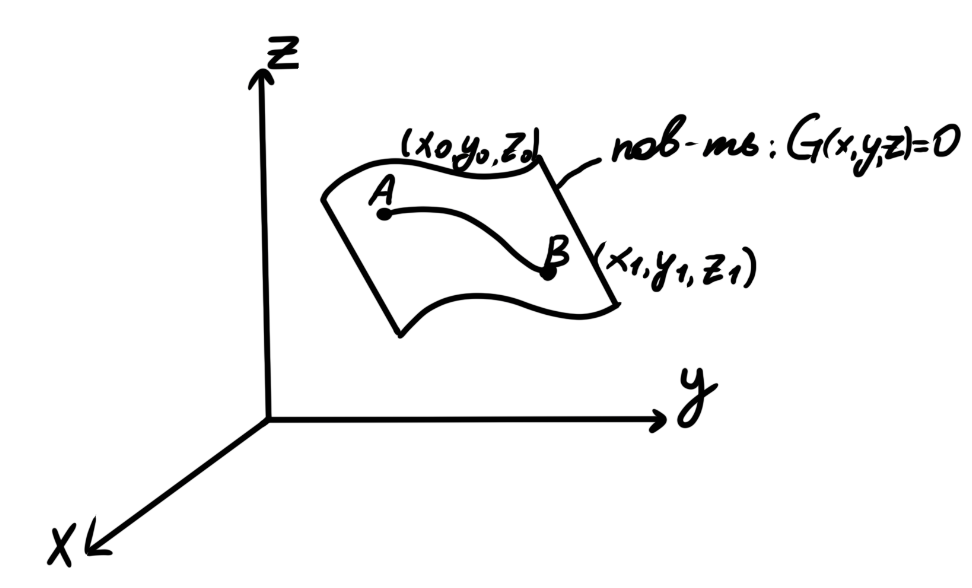
\includegraphics[width=0.5\textwidth]{/Users/vladbelousov/Desktop/Semestr_4-FP-NSU/ДфУ/Лекции_по_дням/image/19.png}
\end{center}

Найти кривую, соединяющую точки A и B, лежащие на поверхности, имеющую наименьшую длину. 

\[ \begin{cases}
x = x(t ) \\
y = y(t ) \quad  \text{уравнение кривой в параметрическом виде } ,\text{ }  t \in [t_0 , t_1]\\
z = z(t )
\end{cases} \] 

\[ I [x,y,z]  = \int_{t_0}^{t_1} \sqrt{(x' (t )) ^2 + (y' (t )) ^2 + (z' (t )) ^2 }dt \] 

\[\begin{cases}
x(t_0 ) = x_0 ,\quad x(t_1 ) = x_1 \\
y(t_0 ) = y_0 ,\quad y(t_1 ) = y_1 \\
z(t_0 ) = z_0 ,\quad z(t_1 ) = z_1
\end{cases} \] 

\textbf{Необходимое условие локального экстремума}:

Пусть \( \tilde{y_1 }, ..., \tilde{y }_n  \)  доставляют локальному экстремум для задачи (1). Тогда \( \exists    \lambda(t)   \) такая, что функции \( \tilde{y_1 }, ..., \tilde{y }_n  \) являются экстремалями вспомогательного функционала. 

\[ \tilde{I } [y_1, \ldots, y_n ] = \int_{t_0}^{t_1} (F + \lambda G(t))dt  \] 

\textbf{Без доказательства.} 

\section{Решение задачи о геодезических на сфере}

\begin{center}
    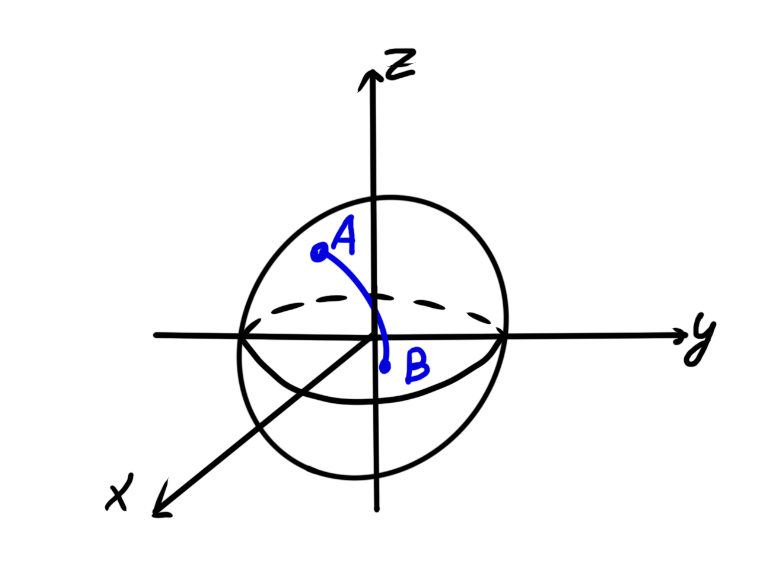
\includegraphics[width=0.4\textwidth]{/Users/vladbelousov/Desktop/Semestr_4-FP-NSU/ДфУ/Лекции_по_дням/image/20.png}
\end{center}

\[ x ^2  +y ^2 + z ^2 = R ^2  \] 

\[ I [x,y,z] = \int_{t_0}^{t_1} \sqrt{(x' (t )) ^2 + (y' (t )) ^2 + (z' (t )) ^2 }dt \] 

\[ \tilde{I } [x,y ,z ] = \int _{t_0}^{t_1}  \underbrace{\left(  \underbrace{\sqrt{(x' (t )) ^2 + (y' (t )) ^2 + (z' (t )) ^2 }}_{F}  + \lambda(t)(x ^2  +y ^2 + z ^2 - R ^2 ) \right)}_{\tilde{F}}  dt  \] 

\[\begin{cases}
    \displaystyle 2 x \lambda (t ) = \frac{d}{dt } \left( \frac{x' }{F}  \right) \quad (1)   \\
    \displaystyle 2 y \lambda (t ) = \frac{d}{dt } \left( \frac{y' }{F}  \right)  \quad (2)\\
    \displaystyle 2 z \lambda (t ) = \frac{d}{dt } \left( \frac{z' }{F}  \right) \quad (3)
\end{cases} \] 

\[ \begin{cases}
    \displaystyle (1) \cdot y + (2) \cdot (-x):\quad  y \frac{d}{dt } \left( \frac{x' }{F} \right) -x \frac{d}{dt } \left( \frac{y' }{F} \right) = 0 \\
    \displaystyle (2) \cdot z + (3 ) \cdot (- y) :\quad z \frac{d}{dt } \left( \frac{y' }{F} \right) -y \frac{d}{dt } \left( \frac{z' }{F} \right) = 0 \\
    \displaystyle (3) \cdot (-x) + (1) \cdot  z : \quad z \frac{d}{dt } \left( \frac{x' }{F} \right) -x \frac{d}{dt } \left( \frac{z' }{F} \right) = 0 
\end{cases} \] 

\[ \frac{d}{dt } \left( y \frac{x ' }{F }  - x \frac{y '}{F}  \right) = \cancelto{0}{y ' \frac{x ' }{F }} + y \frac{d}{dt } \left( \frac{x' }{F}  \right) \cancelto{0}{- x ' \frac{y '}{F}} - x \frac{d}{dt } \left( \frac{y' }{F}  \right) \] 

\[
\begin{aligned}
    \begin{cases}
        \displaystyle \frac{d}{dt } \left( y \frac{x' }{F } - x \frac{y ' }{F}  \right) = 0 \\
        \displaystyle \frac{d}{dt } \left( z \frac{y' }{F } - y \frac{z' }{F}  \right) = 0 \\
        \displaystyle \frac{d}{dt } \left( z \frac{x' }{F } - x \frac{z ' }{F}  \right) = 0 
    \end{cases} 
    \begin{cases}
        \displaystyle \frac{y x' - x y ' }{F } = c_1  \quad (1)\\
        \displaystyle \frac{z y' - y z ' }{F } = c_2  \quad (2)\\ 
        \displaystyle \frac{z x' - x z ' }{F } = c_3 \quad (3)
    \end{cases}
\end{aligned}\] 



\[ (1 )  \cdot z + (2)\cdot x + (3 ) \cdot (-y) : \]

\[ \frac{1}{F} \left[ z(y x' - x y ' ) + x (z y' - y z ' ) - y(z x' - x z ' ) \right] = c_1 z + c_2 x -  c_3 y  \] 

\[ \begin{cases}
    c_1 z + c_2 x -  c_3 y =  0 - \text{плоскость проходящая через (0,0,0)} \\
    x ^2 + y ^2 + z ^2 = R ^2 
\end{cases}  \] 

\begin{center}
    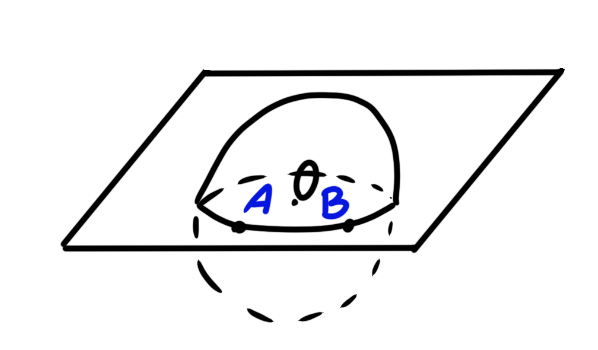
\includegraphics[width=0.3\textwidth]{/Users/vladbelousov/Desktop/Semestr_4-FP-NSU/ДфУ/Лекции_по_дням/image/21.png}
\end{center}

Геодезическая на сфере - дуга на большой окружности.

\chapter{Система малых колебаний}

\section{Линейные однородные системы малых колебаний}

\[ M \vec{x''}  + K \vec{x}  = 0  \quad  (1) \] 

\[ \vec{x }  =\vec{x } (t) = \begin{pmatrix}
x_1( t)\\
\vdots\\
x_n (t)
\end{pmatrix} \quad  M =\begin{pmatrix}
m_{11} & ... & m_{1n}\\
\vdots &  & \vdots\\
m_{n_1} & ... & m_{nn} 
\end{pmatrix} \quad K=\begin{pmatrix}
    k_{11} & ... & k_{1n}\\
    \vdots &  & \vdots\\
    k_{n_1} & ... & k_{nn} 
\end{pmatrix}  \]

Пример: \( n =1 \Rightarrow m x'' + kx = 0 , \text{ } m >0 , \text{ } k > 0 \) 

\begin{center}
    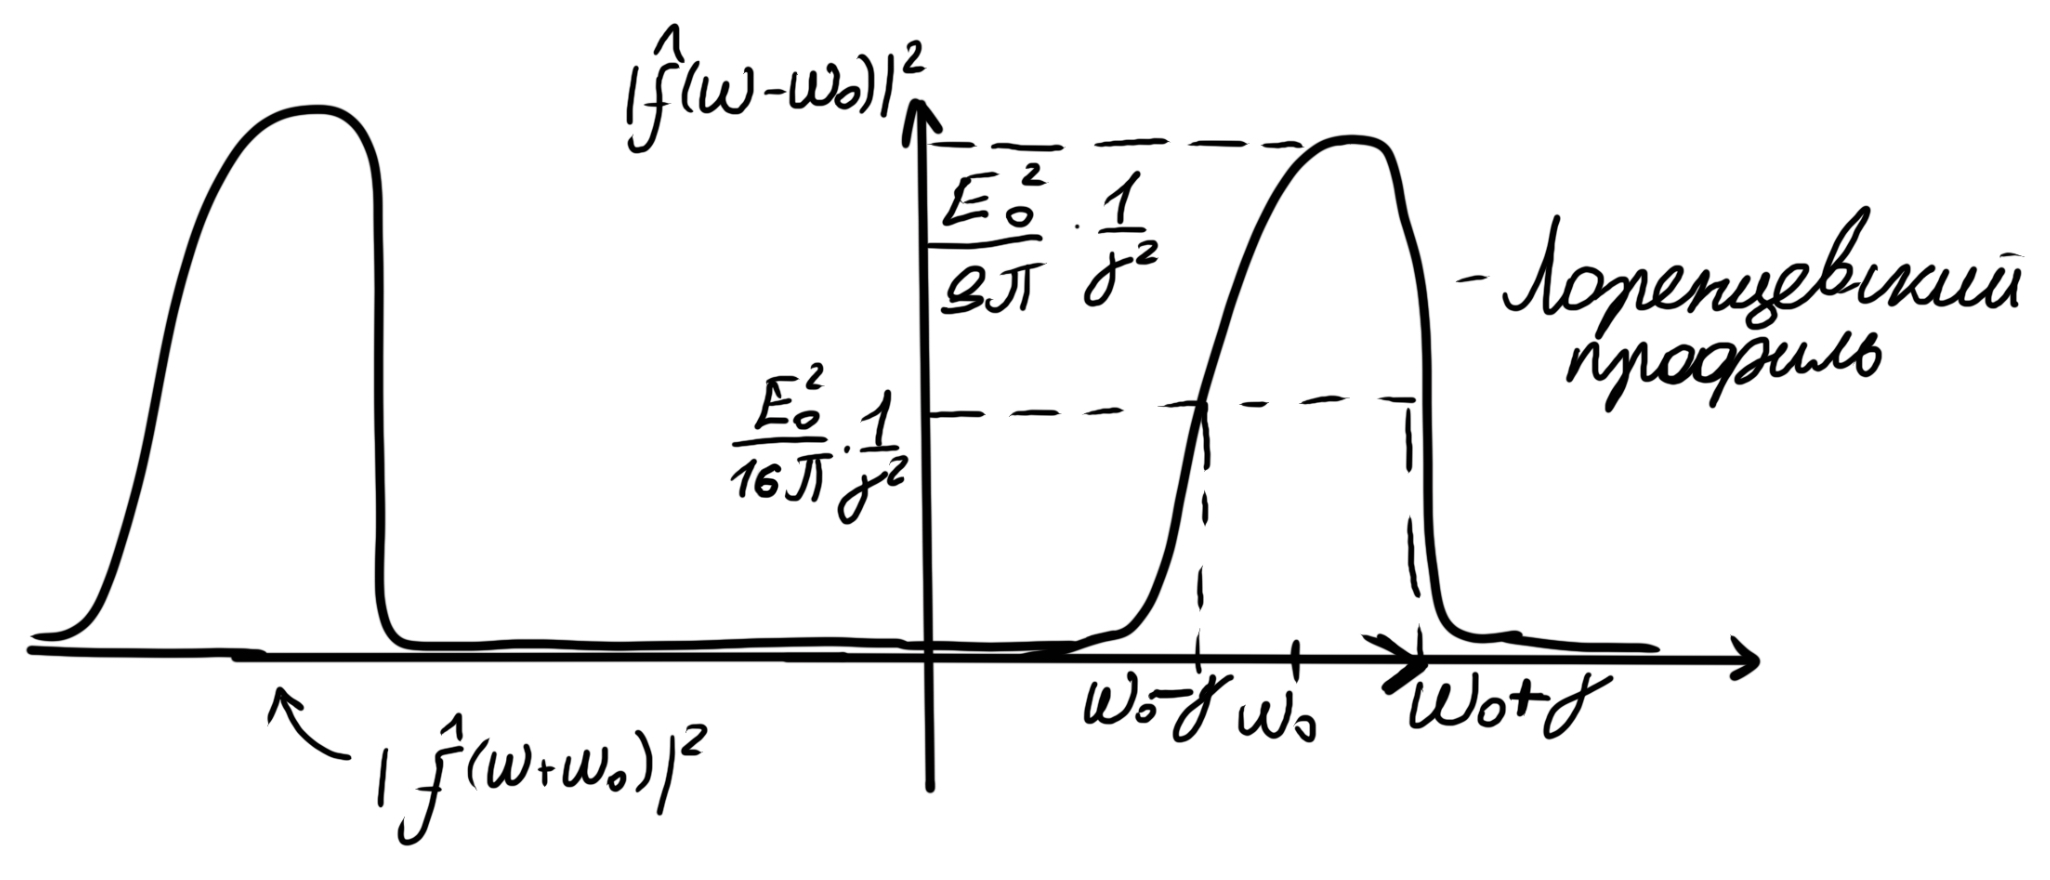
\includegraphics[width=0.3\textwidth]{/Users/vladbelousov/Desktop/Semestr_4-FP-NSU/ДфУ/Лекции_по_дням/image/22.png}
\end{center}

\[ M -\text{ матрица масс} , \quad  K -\text{ матрица жесткостей } \] 

1) \( M = M^{\top} , \text{ }  K = K^{\top}   \text{ } (m_{ij}= m_{j i} ,\text{ } k_{ij} = k_{j i}   ) \) 

2) M > 0  (матрица положительна определена), \( K \geq 0 \) 

\begin{definition}
    Матрица \( M = M^{\top} \) называется положительно определенной, если \( \forall \vec{v } \in  \mathbb{R} ^{n } , \vec{v } \neq 0  \) выполняется \( (M\vec{v} , \vec{v} ) >0 \).  
\end{definition}

\textbf{Критерий Сильвестра: } \( M = M^{\top} > 0 \Leftrightarrow  \text{все главные миноры} > 0. \)

\textbf{1-ый способ:} Сведение к системе 1-го порядка. 

\[ \begin{aligned}
    \begin{cases}
        \vec{y_1 } = \vec{x } \\
        \vec{y_2 } = \vec{x '} 
    \end{cases}
    \begin{cases}
        \vec{y_1 '} = \vec{y_2} \\
        \vec{y_2  '} = \vec{x ''} = -M ^{-1} K \vec{x }  = - M ^{-1} K \vec{y_1}   
    \end{cases}
\end{aligned} \] 

\[ \frac{d}{dt} \begin{pmatrix}
\vec{y_1} \\
\vec{y_2} \\
\end{pmatrix} = \underbrace{\overbrace{\begin{pmatrix}
    0 &  & E\\
     &  & \\
    -M^{-1}K  &  & 0
    \end{pmatrix}}^{A}}_{n \times n}  \begin{pmatrix}
\vec{y_1} \\
\vec{y_2} \\
\end{pmatrix}   \] 





\[ \begin{pmatrix}
    \vec{y_1} \\
    \vec{y_2} \\
\end{pmatrix} =\underbrace{e^{t A }}_{(2n \times  2n)} \underbrace{\vec{c}}_{(2n \times  1)}  = \begin{pmatrix}
\Phi_{11}(t) & \Phi_{12}(t)\\
\Phi_{12}(t) & \Phi_{22}(t)
\end{pmatrix} \begin{pmatrix}
\vec{c_1} \\
\vec{c_2} 
\end{pmatrix}  \]

\[ \vec{x} (t ) = \vec{y_1 } (t ) = F_{11} (t ) \vec{c_1 }  + F_{12} (t ) \vec{c_2 } \quad  (\text{2n констант} )    \] 

\begin{lemma}
    Если \( M = M^{\top} > 0  \), то \( \exists  M^{-1}  \)  
\end{lemma}

\begin{proof}
    \[  \] 
    Пусть не существует \( M^{-1} \Rightarrow \kern-30pt\underbrace{\mathrm{det } M = 0}_{\displaystyle \underset{ \displaystyle \det (M - 0 E) = 0}{\Rightarrow \lambda = 0 - \text{собств.знач.} }}\kern-30pt \Rightarrow \exists  \vec{v } \neq 0 : M \vec{v } = 0  \) 

    \[ (M\vec{v } , \vec{v }     ) = (0, \vec{v } ) = 0 - \text{  противоречие}  \] 
\end{proof}


\begin{proposition}[из алгебры]
    Пусть \( A = A^{\top} \Rightarrow  \)  все собственные числа \( \lambda_j \in  \mathbb{R}.  \) 

    Пусть  \( A = A^{\top} > 0 \Rightarrow  \) все собственные числа \( \lambda_j > 0.  \)
\end{proposition}

\begin{proposition}[из алгебры]
    Пусть \( A = A^{\top} \Rightarrow   \) в \( \mathbb{R} ^n  \)  существует базис из собственных векторов, то есть нет присоединенных 
\end{proposition}

\begin{proposition}[из алгебры]
    Пусть \( A = A^{\top} \Rightarrow A = U D U^{-1}  \), \( \begin{pmatrix}
    \lambda_1 &  & 0\\
    &\ddots  & \\
    0& & \lambda_n
    \end{pmatrix} \) 

\( U  \) - ортогональная  матрица, то есть \( U ^{-1} = U^{\top }   \)  
    
\end{proposition}

\textbf{2-ой способ:}

\begin{definition}
    Число \( \lambda     \)  называется собственным числом системы (1), если
    
    \( \det (K -\lambda M ) = 0 \) 
\end{definition}

\begin{definition}
    Вектор \( \vec{v }  \neq \vec{0}  \)  называется собственным вектором системы (1) (вектором нормальных колебаний), если \( (K -\lambda M ) \vec{v } = 0 \) 
\end{definition}

\begin{theorem}
    Существует n собственных чисел системы (1) и \( \lambda_{i } \geq 0 , \forall  i = 1,2,...,n \) 
\end{theorem}

\begin{proof}
\[  \]

1) \( \det (K -\lambda M )  = 0 \) 

\[ \det (M(M^{-1} K - \lambda E )) = 0 \] 

\[ \underbrace{\det M}_{ \neq 0} \det (M^{-1 } K - \lambda E ) = 0 \Rightarrow \text{ существует n собственных чисел}  \] 

2) \( \vec{v_j}  \)  - собственные вектора \( \Rightarrow K \vec{v_j} = \lambda_j M \vec{v_j} \text{ } | \cdot \vec{v_j}   \)  

\[ \underbrace{(K v_{j }  , v_j)}_{\geq 0}  = \lambda_j \underbrace{(M v_j ,v_j)}_{>0} \Rightarrow \lambda_j \geq 0  \] 
\end{proof}

\begin{theorem}
    В \( \mathbb{R} ^n \)  существует базис из собственных векторов системы (1).
\end{theorem}

\textbf{Доказательство будет позже.} 

\begin{theorem}
    Пусть  \( M = M^{\top} > 0 , K =K ^{\top} \geq 0 , \lambda_1, \ldots, \lambda_n \geq 0 \)  - собственные числа системы (1), \( \vec{v_1 },..., \vec{v_n}   \)  - собственные вектора системы (1), соответвующие числам \( \lambda_1, \ldots, \lambda_n \). Тогда все решения системы (1)  имеют вид: 

    \[ x(t) = \sum_{j=1} ^{n } q_j (t)\vec{v_j},   \] 

    , где \( q_j(t) \)  - решение дифференциального уравнения: \( q_j '' + \lambda_j q_j = 0 \) 
\end{theorem}

\begin{proof}
    \[  \] 
    По теореме 2 \( \vec{v_1},..., \vec{v_n }   \)  - базис в \( \mathbb{R} ^ n \). При фиксированном t \( x(t ) \in  \mathbb{R}^{n} \Rightarrow \vec{x } (t)  \)  раскладывается по базису: \( \vec{x } (t) = \sum_{j=1} ^{n } q_j (t)\vec{v_j}  \) 

    Подставляем \( x(t) \)  в систему (1): 

    \[ M \sum_{j =1}^n q_j '' (t ) \vec{v_j} + K \sum_{j =1}^n q_j (t ) \vec{v_j} = 0  \] 

    \[ \sum_{j=1}^ n \left( q_j '' (t ) M \vec{v_j } + q_j (t )\underbrace{ K \vec{v_j } }_{\lambda_j M \vec{v_j } } \right) =0\] 

    \[ \sum _{j=1}^ n \left( q_j '' (t ) M \vec{v_j } + \lambda_j q_j (t )M\vec{v_j }  \right) = 0 \text{ }  | \cdot  M^{-1}  \] 

    \[ \sum _{j=1}^ n \left( q_j '' (t  ) + \lambda_j q_j (t ) \right) \vec{v_j }= 0 , \text{ }  \forall  t \in  \mathbb{R}   \] 

    \[ \text{Т.к } \vec{v_1 },..., \vec{v_n} \text{ линейно независимы, то }  q_j '' (t ) + \lambda_j q_j (t) =0    \] 


\end{proof}

\begin{center}
    \textbf{Замечание.} \( q_j ''(t ) + \lambda_j q_j (t) = 0 \) 
    1) \( \lambda_j = 0 \Rightarrow q_j (t ) = c_1 t + c_2  \) 

    2) \( \lambda_j > 0 \Rightarrow q_j (t )  = c_1 \cos (\sqrt{\lambda_j} t) + c_2 \sin (\sqrt{\lambda_j} t) \)
\end{center}

\begin{definition}
    \( \omega_1 = \sqrt{\lambda_1},..., \omega_n = \sqrt{\lambda_n} \) называется собственными частотами колебаний системы (1).
\end{definition}

%%-------------------------------%%

% Закрытие документа, если файл компилируется отдельно
\ifdefined\mainfile
    % Если это основной файл, не нужно заканчивать документ
\else
    \end{document}
\fi